\section{$M_{eff}$ as an alternative variable choice to $H_{T}$}

$H_{T}$ was chosen for the eta-HT kinematic method as SM processes dominate in the low region, whilst potential SUSY signal can dominate in the higer regions. Another observable which exhibits these characteristics is $M_{eff}$, the sum of $H_{T}$ and $MHT$. We repeat the same analysis as before, using regions of $M_{eff}$ to study $R_{\alpha_{T}}$, having first applied a baseline cut of $H_{T} >$ 350. For this study, we use the same data samples as in the main section, with the exception of the QCD madgraph and $\mathrm{b \bar{b}}$. For these processes we now use a Pythia6 QCD simulation, generated in lower-limit $\hat{p_{T}}$ bins described in Table~\ref{tab:pyth}.As these are inclusive files, care has been taken to remove over-laps. 

\begin{table}[h!]
\centering
\begin{tabular}{|c||c||c|}
\hline
Lower $\hat{p_{T}}$ limit & Number MC Evts & $\sigma$ \\
\hline
\hline
80 GeV & 3477680 & 1934639.6 \\ 
\hline
170 GeV & 3756780 & 62562.9 \\ 
\hline
300 GeV & 1815585 & 3664.6 \\
\hline
470 GeV & 2426752 & 315.5 \\ 
\hline
800 GeV & 2832476 & 11.9 \\ 
\hline
1400 GeV & 584256 & 0.172 \\ 
\hline
2200 GeV & 878796 & 0.00142 \\ 
\hline
3000 GeV & 567040 & 0.0000086 \\
\hline
\end{tabular}
   \caption{\small{\textit{Number of events generated and cross-sections for the Pythia6 QCD Monte Carlo datasets used.They have been generated in inclusive bins with lower limits in $\hat{p_{T}}$. For the study we have taken care to remove all over-laps due to the inclusive binning}}}
 \label{tab:pyth} 
\end{table}

Figure \ref{fig:meff1} displays the distribution of $M_{eff}$ for all the SM backgrounds and the SUSY signal (LM0 and LM1), after the steps of standard selection up to the $\alpha_{T}$ cut. The relationship between SUSY signal and SM background processes clearly changes in the different regions of $M_{eff}$. While background processes clearly dominate for low values, as we increase in $M_{eff}$ they diminish, while signal distributions are still high. Regions of $M_{eff}$ should therefore have largely differing values for $R_{\alpha T}$.


\begin{figure}[h!]
%\begin{minipage}[b]{0.5\linewidth} % A minipage that covers half the page
\centering
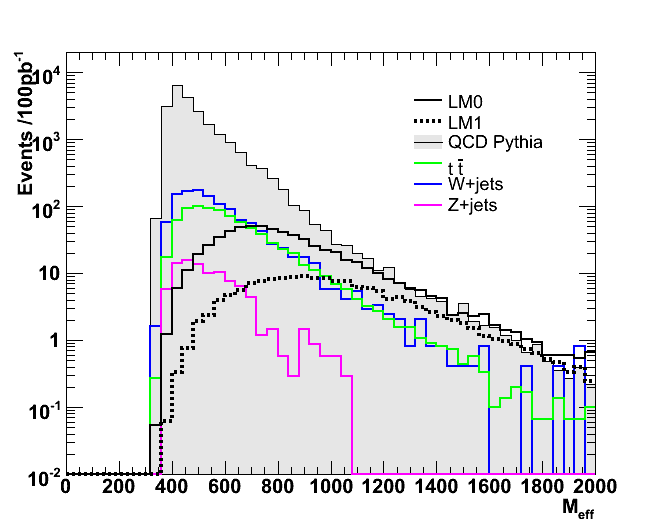
\includegraphics[scale=0.3]{./plots/Meff-NT7-Dist.png}
%\end{minipage}
%\hspace{0.1cm} % To get a little bit of space between the figures
%\begin{minipage}[b]{0.5\linewidth}
%\centering
%\includegraphics[scale=0.4]{}
%\end{minipage}
\caption{\small{\textit{The $M_{eff}$ distribution for the LM0 and LM1 SUSY signal and all the SM backgrounds superimposed, for an intergrated luminosity of 100pb$_{-1}$.}}}
\label{fig:meff1}
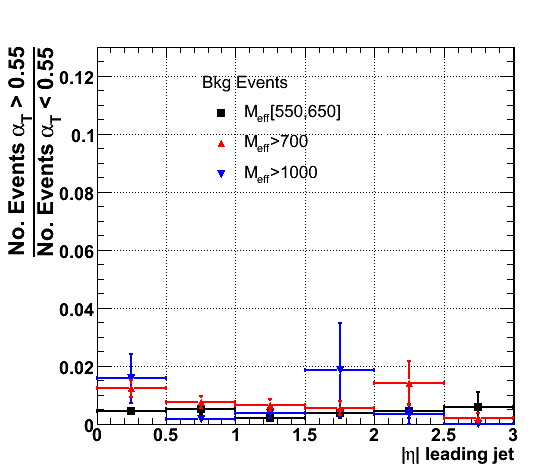
\includegraphics[scale=0.4]{./plots/Meff-NT7-Bkg-MCerr}
%\end{minipage}
%\hspace{0.1cm} % To get a little bit of space between the figures
%\begin{minipage}[b]{0.5\linewidth}
%\centering
%\includegraphics[scale=0.4]{}
%\end{minipage}
\caption{\small{\textit{The $R_{\alpha T}$ versus the leading jet $|\eta|$ for the SM background-only hypothesis, in three $M_{eff}$ bins [550, 650], [700, inf], [1000, inf].} }}
\label{fig:meff2}
\end{figure}

Figure \ref{fig:meff2} shows the $R_{\alpha T}$ versus the $|\eta|$ of the leading jet for the SM background only case, in three chosen regions of $M_{eff}$. The lowest is an exclusive bin with upper and lower limits to choose control region only, and in addition two inclusive bins with lower limits only. The distribution of $R_{\alpha T}$ in this background-only hypothesis is flattish for all regions, as in the $H_{T}$ case. This is expected as for background processes the leading jet has little predisposition to centrality. 
In figures \ref{fig:meff3}, we plot the value of $R_{\alpha T}$ for the SUSY signal LM0 (left) and LM1 (right) respectively, plus the SM background, versus $|\eta|$ of the leading jet. Comparing these to the background-only hypothesis, it can be seen a significant deviation occurs, increasing in Meff bins. The signal case is more central than the background-only, and this is more pronounced as we move to higher regions of $M_{eff}$, where the signal is more prominent against background. 

Comparing these to the $H_{T}$ case, we see the same characteristics. Numerically the gain in $R_{\alpha T}$ is on a greater scale than that seen in the $H_{T}$ case, but the errors are larger too. In order to inspect the deviation quantitatively, the $R_{\alpha T}$ distribution is fitted, as previously done for HT. The $R_{\alpha T}$ vs the $|\eta|$ of ther leading jet is fitted with a 1st degree polynomial ($p0+p1.|\eta|$) using the $\chi^{2}$ method. The corresponding plots of the parameters of the fit are seen in Figure~\ref{fig:meff4} for the cases with and without signal. As in the HT case, the background-only picture shows flat distribution in $M_{eff}$ for both p0 and p1, while the SUSY signal is much more pronounced in regions of high $M_{eff}$ than in the low control region. It can also be seen that for LM0, the deviation from the background picture reaches a plateau at 750 GeV while for LM1 it continues. This is inherent from the mass spectrum of the LM0 case. 
\begin{figure}[h!]
\begin{minipage}[b]{0.5\linewidth}
\centering
{\label{fig:lm0_RaT}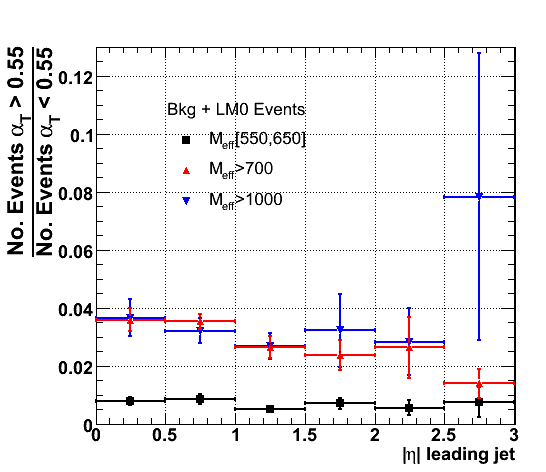
\includegraphics[scale=0.4]{./plots/Meff-NT7-Lm0-MCerr}} 
\end{minipage}
\begin{minipage}[b]{0.5\linewidth}
\centering
{\label{fig:lm1_RaT}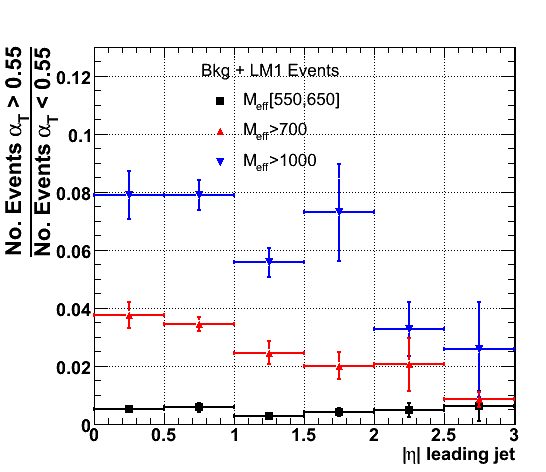
\includegraphics[scale=0.4]{./plots/Meff-NT7-Lm1-MCerr}} 
\end{minipage}
\caption{\small{\textit{The $R_{\alpha T}$ versus the leading jet $|\eta|$ for the SUSY signal (LM0 on the left, LM1 on the right) plus SM background hypothesis, in three $M_{eff}$ bins [550, 650], [700, inf], [1000, inf].} }}
\label{fig:meff3}
\end{figure}


\begin{figure}[h!]
\begin{minipage}[b]{0.5\linewidth}
\centering
{\label{fig:meff_p0}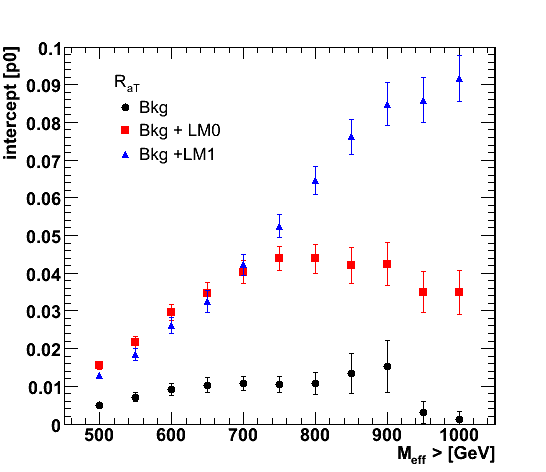
\includegraphics[scale=0.4]{./plots/Meff-NT7-p0-MCerr}} 
\end{minipage}
\begin{minipage}[b]{0.5\linewidth}
\centering
{\label{fig:meff_p1}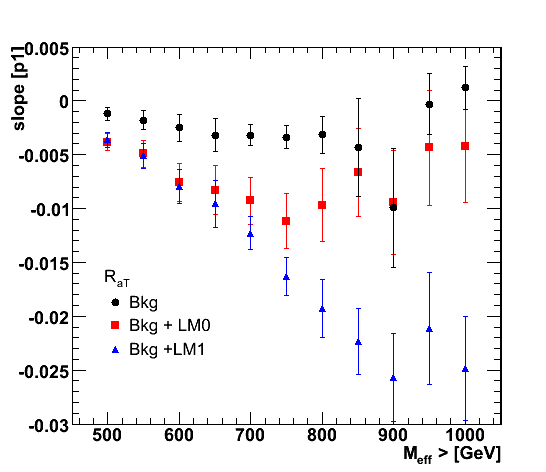
\includegraphics[scale=0.4]{./plots/Meff-NT7-p1-MCerr}} 
\end{minipage}
\caption{\small{\textit{The parameters p0(left) and p1(right) of the first-degree polynomial fit to the $R_{\alpha T}$ versus $|\eta|$ curves, for each value of lower $M_{eff}$ limit [GeV]. Each plot shows three scenarios: background-only hypothesis, and background with added LM0/LM1 signal.}}}
\label{fig:meff4}
\end{figure}


In order to compare the use of $M_{eff}$ in this method to that of HT, we again calculate the quantity $\Delta p_{i} / \sigma$, to consider the significance of the difference between the parameters with and without LM1 signal. Figures~\ref{fig:meff5} and \ref{fig:meff6} show the intercept and gradient plots for Meff (left) against the same plots for HT (right) for comparison. It can be seen that the significance of the intercept increases faster for $M_{eff}$ than for HT, but the corresponding plots for the gradient indicate that using $M_{eff}$ in this method produces less stable results. 

From these plots we can conclude that increasing lower limits in $M_{eff}$ allow a change from a region where SM processes dominate to where SUSY signal is prolific. Thus this variable can be used instead of HT along with $|\eta|$ to establish a deviation from the Standard Model. The deviation apears more pronounced than for the HT method, but significance plots show a more erratic behaviour. Until this behaviour is understood, and can be controlled, more reliable results will be seen with the HT method. 




 




\begin{figure}[h!]
\begin{minipage}[b]{0.5\linewidth}
\centering
{\label{fig:meff_p0_s}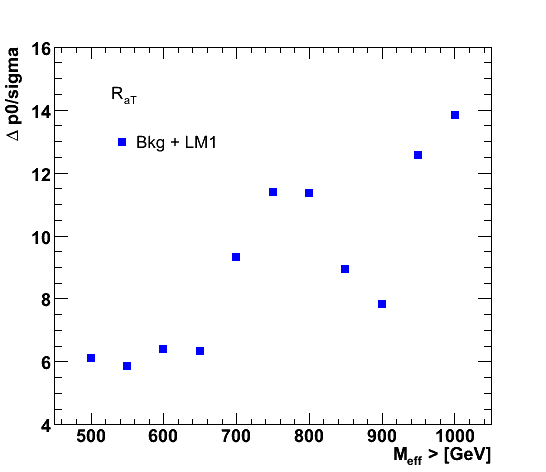
\includegraphics[scale=0.4]{./plots/Meff-NT7-p0-Sig}} 
\end{minipage}
\begin{minipage}[b]{0.5\linewidth}
\centering
{\label{fig:HT_p0_s}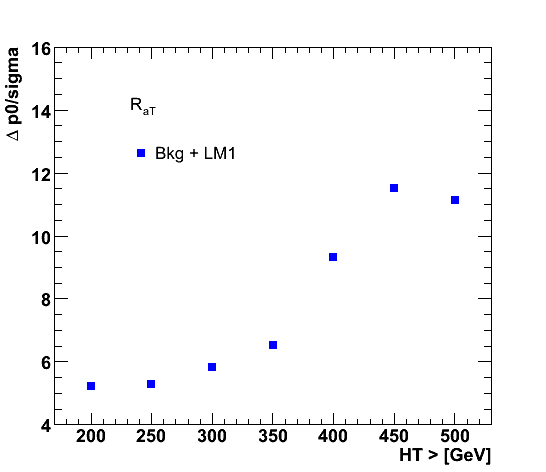
\includegraphics[scale=0.4]{./plots/HT-NT7-p0-Sig}} 
\end{minipage}
\caption{\small{\textit{ $\Delta p_{i} / \sigma$ of the parameter p0 of the fit to the $R_{\alpha T}$ vs. $|\eta|$ plots for $M_{eff}$ (left) and $H_{T}$ (right). This is a measure of 'significance' for establishing a SUSY deviation to the SM-only hypothesis using this parameter.}}}
\label{fig:meff5}
\end{figure}



\begin{figure}[h!]
\begin{minipage}[b]{0.5\linewidth}
\centering
{\label{fig:meff_p1_s}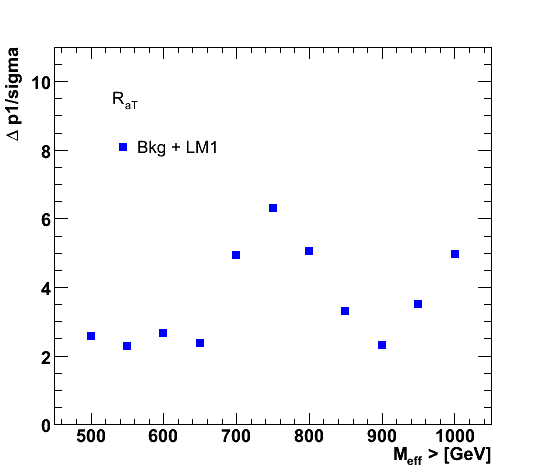
\includegraphics[scale=0.4]{./plots/Meff-NT7-p1-Sig}} 
\end{minipage}
\begin{minipage}[b]{0.5\linewidth}
\centering
{\label{fig:HT_p1_s}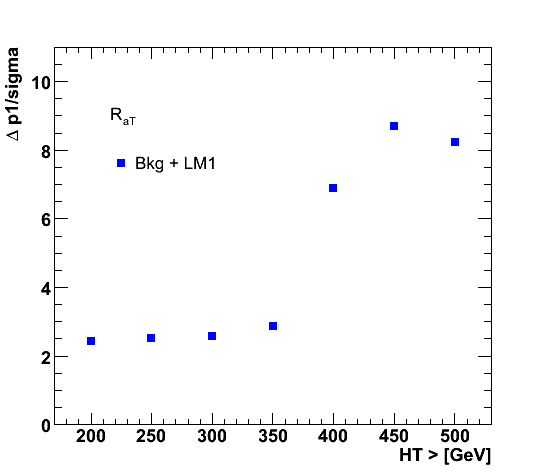
\includegraphics[scale=0.4]{./plots/HT-NT7-p1-Sig}} 
\end{minipage}
\caption{\small{\textit{ $\Delta p_{i} / \sigma$ of the parameter p1 of the fit to the $R_{\alpha T}$ vs. $|\eta|$ plots for $M_{eff}$ (left) and $H_{T}$ (right). This is a measure of 'significance' for establishing a SUSY deviation to the SM-only hypothesis using this parameter.} }}
\label{fig:meff6}
\end{figure}
